\documentclass[tikz,border=6pt]{standalone}
\usepackage{amsmath}
\usetikzlibrary{arrows.meta,positioning,calc,shapes.geometric}

\tikzset{
  >={Latex[length=2.2mm]},
  thick/.style={line width=0.9pt},
  sum/.style   = {draw, circle, inner sep=0pt, minimum size=5mm, thick},
  block/.style = {draw, thick, minimum height=10mm, minimum width=18mm, align=center},
  sblock/.style= {draw, thick, minimum height=7mm, minimum width=12mm, align=center},
  amp/.style   = {draw, thick, isosceles triangle, isosceles triangle apex angle=60,
                  minimum width=10mm, minimum height=9mm, inner sep=0pt},
  sat/.style   = {block, minimum width=18mm, minimum height=11mm},
  wide/.style  = {draw, thick, minimum height=28mm, minimum width=72mm, align=left, inner xsep=8mm},
  tap/.style   = {circle, fill, inner sep=1.2pt}
}

\begin{document}
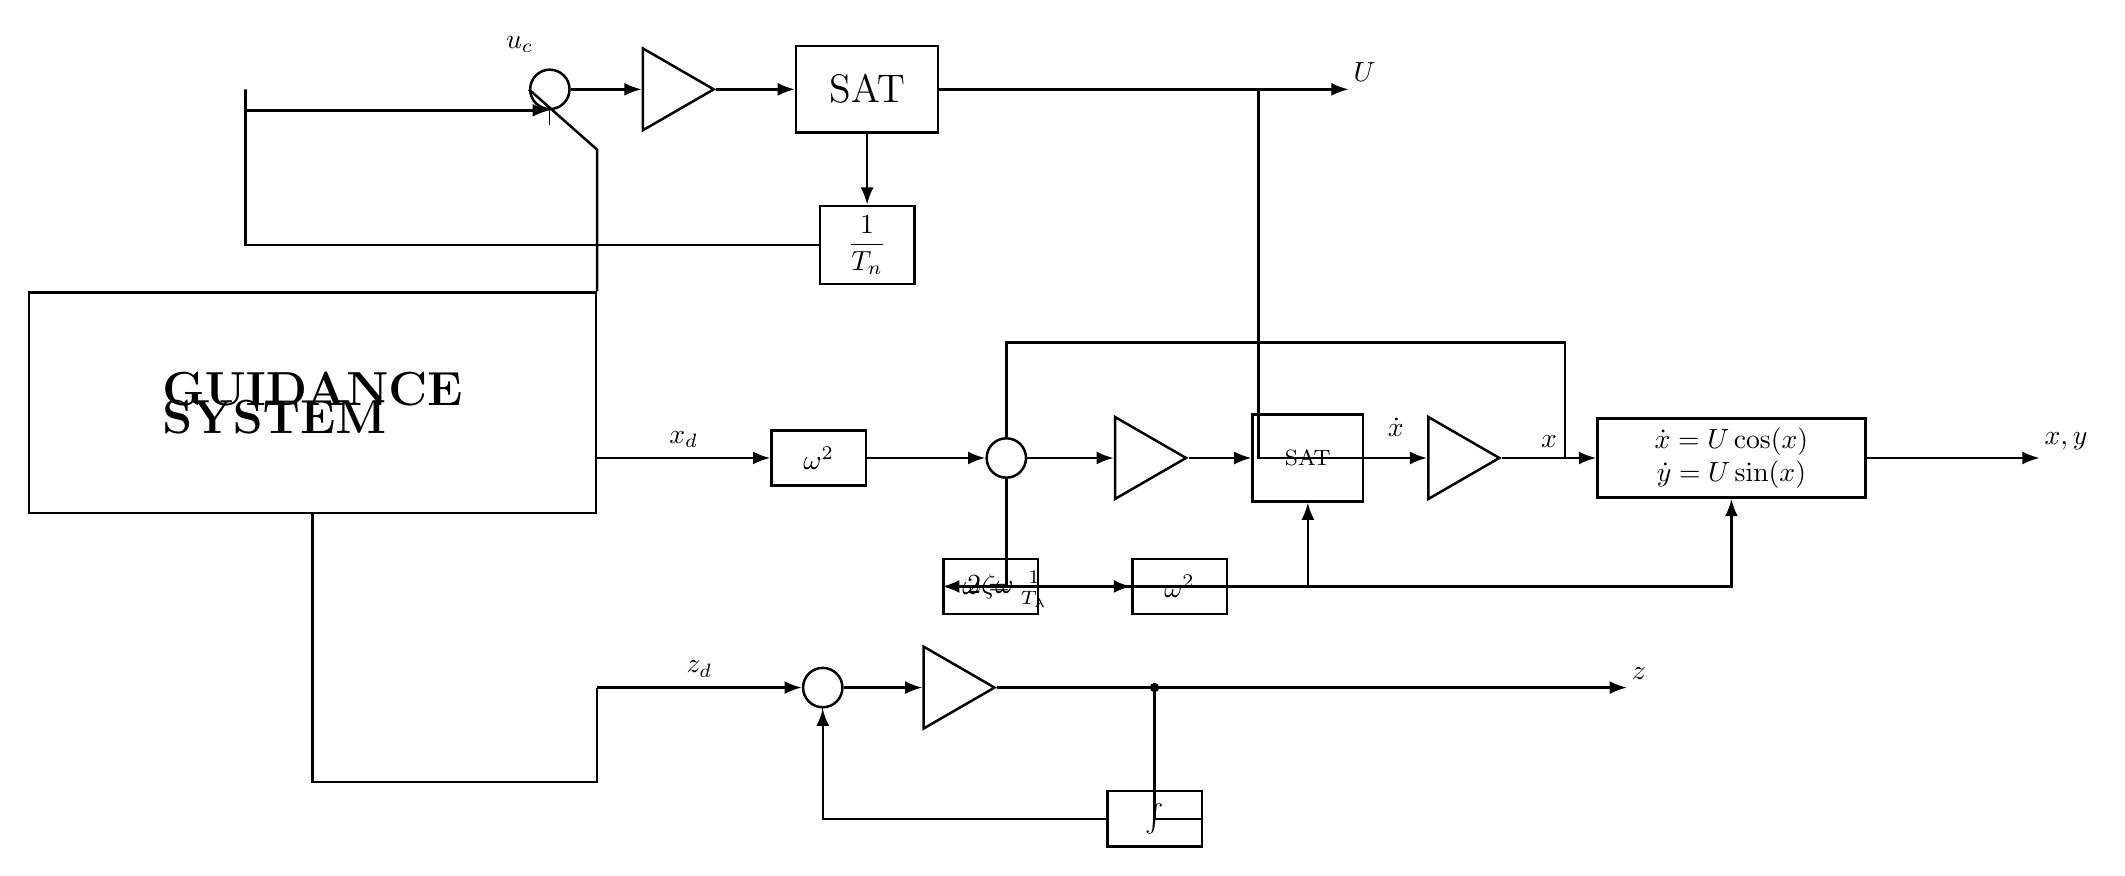
\begin{tikzpicture}[node distance=10mm and 12mm]

%==================== GUIDANCE ====================
\node[wide] (guid) at (0,0) {\LARGE\bfseries GUIDANCE\\[-2pt]\LARGE\bfseries SYSTEM};

%==================== TOP LOOP (U) ====================
\node[sum, above=23mm of guid.north east, xshift=-6mm] (su) {};
\node[above left=1.5mm and -1mm of su] {$u_c$};
\draw ($(su.center)+(0,-2.5mm)$) -- ++(0,-2mm); % minus

\node[amp, right=9mm of su] (au) {};
\node[sat, right=10mm of au] (satU) {\Large SAT};
\node[sblock, below=9mm of satU] (intU) {$\dfrac{1}{T_n}$};

\coordinate (Uout) at ($(satU.east)+(52mm,0)$);
\draw[->,thick] (satU.east) -- (Uout) node[above right=-1pt and -2pt] {$U$};
\coordinate (Utap) at ($(satU.east)!0.78!(Uout)$); % hvor vi tapper U
\draw[thick] (Utap) -- ++(0,-0.5);                 % start på vertikal tapp

\draw[->,thick] (su) -- (au);
\draw[->,thick] (au) -- (satU);
\draw[->,thick] (satU.south) -- (intU.north);
\draw[->,thick] (intU.west) -| ($(su.west)+(-36mm,0)$) |- (su.south);

% kobling fra GUIDANCE opp til summer
\draw[thick] (guid.north east) -- ++(0,18mm) -- (su.west);

%==================== MIDDLE (x, y) ====================
\coordinate (xdL) at ($(guid.east)+(0mm,-7mm)$);
\node[sblock, right=22mm of xdL] (w2in) {$\omega^2$};
\node[sum, right=15mm of w2in] (sx) {};
\node[amp, right=11mm of sx] (ax1) {};
\node[sat, right=8mm of ax1, minimum width=14mm] (satx) {\footnotesize SAT};
\node[amp, right=8mm of satx] (ax2) {};
\node[block, right=12mm of ax2, minimum width=34mm] (kin) {$\dot{x}=U\cos(x)$\\$\dot{y}=U\sin(x)$};
\coordinate (xyout) at ($(kin.east)+(22mm,0)$);

% hovedlinje
\draw[->,thick] (xdL) -- node[above] {$x_d$} (w2in.west);
\draw[->,thick] (w2in.east) -- (sx.west);
\draw[->,thick] (sx) -- (ax1);
\draw[->,thick] (ax1) -- (satx);
\draw[->,thick] (satx) -- (ax2);
\draw[->,thick] (ax2) -- node[above] {$x$} (kin);
\draw[->,thick] (kin.east) -- (xyout) node[above right=-1pt and -2pt] {$x,y$};

% U-tapp til linja MELLOM SAT og høyre amp (ved \dot{x})
\coordinate (xdotPt) at ($(satx.east)!0.5!(ax2.west)$);
\draw[thick] (Utap) |- (xdotPt);
\node[above=1.5mm of xdotPt] {$\dot{x}$};

% state feedback-grener
\node[sblock, below=10mm of sx, xshift=-2mm] (damp) {$2\zeta\omega$};
\node[sblock, below=10mm of sx, xshift=22mm] (w2fb) {$\omega^2$};
\node at ($(sx.south)+(0,-14mm)$) {$\omega=\tfrac{1}{T_\lambda}$};

\draw[->,thick] (sx.south) |- (damp.west);
\draw[->,thick] (sx.south) |- (w2fb.west);
\draw[->,thick] (damp.east) -| (satx.south);
\draw[->,thick] (w2fb.east) -| (kin.south);

% x-tilbake til summerskive (øvre lang retur)
\draw[thick] (ax2.east) -- ++(8mm,0) |- ($(sx.north)+(0,12mm)$) -| (sx.north);

%==================== BOTTOM (z) ====================
\coordinate (zdL) at ($(guid.south east)+(0mm,-22mm)$);
\node[sum, right=26mm of zdL] (sz) {};
\draw ($(sz.center)+(0,-2.5mm)$) -- ++(0,-2mm); % minus
\node[amp, right=10mm of sz] (az) {};
\coordinate (znode) at ($(az.east)+(20mm,0)$);
\node[tap] (ztap) at (znode) {};
\coordinate (zend) at ($(znode)+(60mm,0)$);
\draw[->,thick] (znode) -- (zend) node[above right=-1pt and -2pt] {$z$};

\node[sblock, below=13mm of znode, minimum width=12mm] (intZ) {$\int$};

\draw[->,thick] (zdL) -- node[above] {$z_d$} (sz.west);
\draw[->,thick] (sz) -- (az);
\draw[-,thick]  (az.east) -- (znode);
\draw[thick] (znode) |- (intZ.east);
\draw[->,thick] (intZ.west) -| (sz.south);

% vertikal stamlinje fra GUIDANCE til z-gren
\draw[thick] (guid.south) -- ++(0,-34mm) -| (zdL);

\end{tikzpicture}
\end{document}
